%
% change log:
% originally setting up around the Jan. 2009,
% begin to revise at end of the June.
% 1 revise the Thomas-Fermi model, derive the kinetic energy 23th, June
% 2 derive the exchange energy 24th, June
% 3  change the hbar in the former content into h, correct a bug
% revise from July 8th to 15th, 2009:
% rewrite the whole uniform electron gas analysis, and the discussion with
% kinetic energy and exchange energy
%

\chapter{Functionals in Density Functional Theory}
\label{Functionals_in_DFT}
%%%%%%%%%%%%%%%%%%%%%%%%%%%%%%%%%%%%%%%%%%%%%%%%%%%%%%%%%%%%%%%%%%%%%%%%%%%%

After establishing the main framework of the Kohn-Sham equations,
there's some important work left for us, which is to find the concrete
expression of the $E_{XC}$. This part of work is the essence of DFT
theory, and it's the most important and difficult task that the theory
meets. So in this chapter, we are trying to review this part of work
in general, and most importantly to get the core idea of this part of
work.



%%%%%%%%%%%%%%%%%%%%%%%%%%%%%%%%%%%%%%%%%%%%%%%%%%%%%%%%%%%%%%%%%%%%%%%%%%%%%
\section{General idea for the $E_{XC}$ in DFT}
%
%
%
%
According to the discussion made in the last chapter(\ref{DFTIeq:29}), the
$E_{XC}$ is generally expressed as:
\begin{align}
  \label{FIDFTeq:90}
  E_{XC}[\rho] &= T[\rho] - T_{S}[\rho] + E_{X}[\rho] + E_{C}[\rho]
\nonumber \\
&=
\frac{1}{2}\int^{\lambda = 1}_{\lambda = 0} \int
\left(\frac{1}{r_{12}}\right)
\rho(r_{1})\rho(r_{2})(g_{\lambda}(r_{1},
r_{2})-1)d^{3}r_{1}d^{3}r_{2} d\lambda \nonumber \\
&=\frac{1}{2} \int \left(\frac{1}{r_{12}}\right)
\rho(r_{1})\rho(r_{2})\widetilde{h}(r_{1},
r_{2})d^{3}r_{1}d^{3}r_{2}
\end{align}


This is some important starting point for getting the concrete form
of $E_{XC}$, and it will be used later in the following part of this
chapter.

However, only the general expression in (\ref{FIDFTeq:90}) is not
enough to derive the concrete form of $E_{XC}$. Hence how can we
derive the concrete form of $E_{XC}$?

The first step is the so called ``LDA'' approximation. Generally, 
this model assumes that all the electron densities are homogeneous 
among all the space, so we have $\rho(r)$ as some constant. Finally, 
in the (\ref{FIDFTeq:90}) we can 
integrate over $r_{2}$, that leads to:
\begin{equation}
 \begin{split}
  E_{XC}[\rho] &= \frac{1}{2} \int \left(\frac{1}{r_{12}}\right)
\rho(r_{1})\rho(r_{2})\widetilde{h}(r_{1},
r_{2})d^{3}r_{1}d^{3}r_{2} \\
&= \int d^{3}r_{1} \rho(r_{1}) 
\left\lbrace 
\frac{1}{2}\int  
\left(\frac{1}{r_{12}}\right)\rho(r_{2})\widetilde{h}(r_{1},
r_{2})d^{3}r_{2}
\right\rbrace  \\
&= \int d^{3}r_{1} \rho(r_{1}) v(r_{1})
 \end{split}
 \label{FIDFTeq:91}
\end{equation}
Here we can see that the $\widetilde{h}(r_{1},
r_{2})$ is integrated over $r_{2}$ which implies that the 
exchange-correlation effects are considered in the average way (just like
the HF wave function). This expression is the general exchange-correlation
energy expression for LDA model.

Gnerally speaking, to approach a concrete XC expression means
we need to find some ``simple'' but ``representative'' physical 
model. From this model, perhaps we can get the exact
wave functions and the corresponding energy levels. Then by using
some physical tools such as the statistical method and the
mathematical tricks, we can get the relation between the electron
density and the corresponding energies (for example, the kinetic
energy, exchange energy etc.). By then, the $E_{XC}$ can be gotten.
In the following sections, we will how to do this within LDA 
approximation.

From the discussion in the (\ref{DFTI:1}), we have known that the
$E_{XC}$ is invariant to any nucleus configurations as well as any
electron densities. Hence it can be well expected that if the
general expression of $E_{XC}$ is gotten, then it can be applied to
any chemistry system from the $H_{2}$ molecule to the complex
protein molecules. Therefore, the $E_{XC}$ is universal in this
point.


%%%%%%%%%%%%%%%%%%%%%%%%%%%%%%%%%%%%%%%%%%%%%%%%%%%%%%%%%%%%%%%%%%%%%%%%%%%%%
\section{Local density approximation}
%
%
%
%
Actually there has some physical model which is paradigm for
deriving the exchange-correlation energy, this is the ``uniform
electron gas model''\cite{DFT_PAPERS_GATHERING,
Peter_Fulde_electron_gas}; which is corresponding to the famous
local density approximation (LDA) in density functional theory.

In this model, the electrons are trapped into some periodically
arranged cubic box with volume of $V=l^{3}$, therefore the electron
states repeat from one face of cube to its opposite face. Inside the
box, there has evenly spreaded positive charge background so that
the total system is able to keep to be neutral, so the electrons are
inhabited in some homogeneous medium.  Furthermore, we assume that
there's no potential of $\hat{V}$ inside the box, so the motion of
electrons can be described by free particle wave function.

Since the free electron model requires that the electron density is
constant, then as $l\uparrow$, the number of electrons inside the cube
must also increase so that to make $\frac{N}{V}$ is some
constant. Therefore, in the content below we do not explicitly assign
the average electron density as some function of $r$ if necessary.

Now let's step into mathematical details. Suppose that the box is
located in the direction below:
\begin{equation}
  \label{eq:FIDFTeq:16}
\hat{V} = 0 \quad (0< x, y, z < l)
\end{equation}
And the boundary condition is:
\begin{equation}
  \label{eq:FIDFTeq:17}
 \left\{
  \begin{array}{ll}
    \hat{V}(x+nl,y,z) = \hat{V}(x,y,z), & \hbox{$n = 0, \pm 1, \pm 2 \cdots$} \\
    \hat{V}(x,y+nl,z) = \hat{V}(x,y,z), & \hbox{$n = 0, \pm 1, \pm 2 \cdots$} \\
    \hat{V}(x,y,z+nl) = \hat{V}(x,y,z), & \hbox{$n = 0, \pm 1, \pm 2 \cdots$}
  \end{array}
\right.
\end{equation}
While $n<0$ indicates that the boxes are extending to the negative
direction of the coordinate system.

Now let's consider the wave function for the (\ref{eq:FIDFTeq:16})
and (\ref{eq:FIDFTeq:17}), it should be:
\begin{align}\label{eq:FIDFTeq:18}
\Psi(k_{x}, k_{y}, k_{z}) &= \frac{1}{l^{\frac{2}{3}}}e^{i(k_{x}x+
k_{y}y+k_{z}z)} \nonumber \\
&=\frac{1}{V^{\frac{1}{2}}}e^{i \mathbf{k}\cdot \mathbf{r}}
\end{align}
Here $\mathbf{k}$ is the corresponding wave vector, and it's
related to the principal quantum number:
\begin{equation}\label{eq:FIDFTeq:19}
k_{x}=\frac{2\pi}{l}n_{x} \quad k_{y}=\frac{2\pi}{l}n_{y} \quad
k_{z}=\frac{2\pi}{l}n_{z}
\end{equation}
Where the $n_{x}, n_{y}, n_{z}$ can adopt $0, \pm 1, \pm 2, \cdots$.

The corresponding energy is:
\begin{align}\label{eq:FIDFTeq:20}
E(n_{x}, n_{y}, n_{z}) &= \frac{h^{2}}{8ml^{2}}[(2n)^{2}_{x} +
(2n)^{2}_{y} + (2n)^{2}_{z}] \nonumber \\
&=\frac{h^{2}}{4\pi^{2}}\left[\frac{k_{x}^{2}}{2m} +
\frac{k_{y}^{2}}{2m} + \frac{k_{z}^{2}}{2m}\right]
\end{align}

If we have:
\begin{equation}
  \label{eq:FIDFTeq:49}
  k^{2} = k_{x}^{2} + k_{y}^{2} + k_{z}^{2}
\end{equation}
Then the corresponding energy is converted to:
\begin{equation}
  \label{eq:FIDFTeq:50}
  E_{k} = \frac{\hbar^{2}}{2m}k^{2}
\end{equation}

Now we assume that within the cube of $V$ there are many electrons
resided in, and we can use the statistical method to evaluate the
density.

Firstly, since that there's only finite number of electrons, then
there must have some energy level on which no electrons residing
in. the highest energy level while the electron occupied is called
``Fermi energy'', and it's labeled as $\epsilon_{F}$. Then according
to Fermi-Dirac statistics, the average number of electrons on
certain energy level of $E_{k}$ is:
\begin{equation}
  \label{eq:FIDFTeq:51}
  n_{k} = \frac{1}{e^{\frac{E_{k}-\epsilon_{F}}{k_{B}T}} + 1}
\end{equation}
$k_{B}$ is the Boltzmann's constant. Then we can evaluate the total
electron number as:
\begin{equation}
  \label{eq:FIDFTeq:52}
  N= 2\sum_{k=-\infty}^{k=+\infty}n_{k} =
  2\sum_{k=-\infty}^{k=+\infty}\frac{1}{e^{\frac{E_{k}-\epsilon_{F}}{k_{B}T}}
    + 1}
\end{equation}
Here the multiplier of $2$ is because that each single electron state
is occupied by two electrons with opposite spin.

By the way, through the (\ref{eq:FIDFTeq:51}) the Fermi energy can be
gotten some clear physical interpretation. At absolute zero
temperature, the occupation number is $1$ for energies less than the Fermi
energy and zero for energies greater than the Fermi energy. Such
situation is pictured in the (\ref{FIDFT:1}).

\begin{figure}
\begin{center}
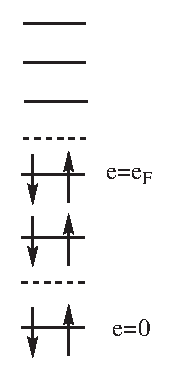
\includegraphics[scale=0.7]{DFT_Fermi.eps}
\caption{Electrons arrangement for uniform electron gas model at $0$k}
\label{FIDFT:1}
\end{center}
\end{figure}

If there are many electron states, then the summation process in
(\ref{eq:FIDFTeq:52}) can be transformed into the integral:
\begin{align}
  \label{eq:FIDFTeq:53}
 N &= 2\int \int \int \frac{1}{e^{\frac{E_{k}-\epsilon_{F}}{k_{B}T}}
    + 1}dn_{x}dn_{y}dn_{z} \nonumber \\
   &= 2\int \int \int \frac{1}{e^{\frac{E_{k}-\epsilon_{F}}{k_{B}T}}
    +
    1}\frac{dk_{x}}{2\pi/l}\frac{dk_{y}}{2\pi/l}\frac{dk_{z}}{2\pi/l}
  \nonumber \\
   &= 2\frac{V}{(2\pi)^{3}}\int \int \int \frac{1}{e^{\frac{E_{k}-\epsilon_{F}}{k_{B}T}}
     + 1}dk_{x}dk_{y}dk_{z}
\end{align}

However, the integration in the (\ref{eq:FIDFTeq:53}) is not
easy to get. Since we only have the energy as some function of
$k_{x}$, $k_{y}$ and $k_{z}$ (see \ref{eq:FIDFTeq:20}), then the
variation for the $k_{x}$, $k_{y}$ and $k_{z}$ are not independent; in
other words, we can not have the integration in the
(\ref{eq:FIDFTeq:53}) transformed into:
\begin{equation}\label{}
\int_{0}^{k_{max}}f(k_{x})dk_{x} \int_{0}^{k_{max}} g(k_{y})dk_{y}\int_{0}^{k_{max}}
h(k_{z})dk_{z}
\end{equation}

For solving this problem, we have to abandon the use the variables
of $(k_{x}, k_{y}, k_{z})$ so that to transform into the sphere
coordinate system of $(k, \theta, \phi$); where $k=\sqrt{k_{x}^{2} +
k_{y}^{2} + k_{z}^{2}}$.

Then we have (\ref{eq:FIDFTeq:53}) becomes:
\begin{equation}\label{eq:FIDFTeq:54}
N = 2\frac{V}{(2\pi)^{3}}
\int_{0}^{k_{F}}\int_{0}^{\pi}\int_{0}^{2\pi}
\frac{1}{e^{\frac{E_{k}-\epsilon_{F}}{k_{B}T}}
+ 1}k^{2}\sin\theta dkd\theta d\phi
\end{equation}

Here $k_{F}$ has very clear physical meaning, it equals to the maximum
value of $k$:
\begin{equation}
  \label{eq:FIDFTeq:55}
  k_{F} = \max \sqrt{k_{x}^{2} + k_{y}^{2} + k_{z}^{2}}
\end{equation}
Hence, $k_{F}$ characterizes the absolute maximum momentum of the wave
functions, it's easy to know that such wave function also gives the
Fermi energy of $\epsilon_{F}$.

Now let's go to see how to express the $k_{F}$. Suppose that it's in
absolute zero temperature, then the (\ref{eq:FIDFTeq:54}) simply
becomes:
\begin{align}
  \label{eq:FIDFTeq:56}
N &= 2\frac{V}{(2\pi)^{3}}
\int_{0}^{k_{F}}\int_{0}^{\pi}\int_{0}^{2\pi}k^{2}\sin\theta dkd\theta
d\phi
\nonumber \\
&= 2\frac{V}{(2\pi)^{3}}
\int_{0}^{k_{F}}k^{2}4\pi dk \nonumber \\
&=\frac{k_{F}^{3}}{3\pi^{2}}V
\end{align}

So far we can see that it's possible for us to associate the electron
density with the $k_{F}$:
\begin{equation}
  \label{eq:FIDFTeq:57}
\rho = \frac{N}{V} = \frac{k_{F}^{3}}{3\pi^{2}}
\end{equation}


%%%%%%%%%%%%%%%%%%%%%%%%%%%%%%%%%%%%%%%%%%%%%%%%%%%%%%%%%%%%%%%%%%%%%%%%%%%%%
\subsection{Kinetic energy derivation}
\label{KED_in_function}
%
%
%
%
Now let's evaluate the kinetic energy through the results above. From
the (\ref{eq:FIDFTeq:51}) and (\ref{eq:FIDFTeq:50}), we can express
the total energy as:
\begin{align}
  \label{eq:FIDFTeq:58}
e_{total} &= 2\sum_{k=-\infty}^{k=+\infty}E_{k}n_{k} \nonumber \\
        &= 2\sum_{k=-\infty}^{k=+\infty}
          \frac{\frac{\hbar^{2}}{2m}k^{2}}{e^{\frac{E_{k}-\epsilon_{F}}{k_{B}T}}
    + 1}
\end{align}

In the large number of wave vectors, the sum can be approximated as
integral (the treatment is similar to the \ref{eq:FIDFTeq:53}):
\begin{align}
  \label{eq:FIDFTeq:59}
e_{total} &= 2\frac{V}{(2\pi)^{3}}\int \int \int
\frac{\frac{\hbar^{2}}{2m}k^{2}}{e^{\frac{E_{k}-\epsilon_{F}}{k_{B}T}}
     + 1}dk_{x}dk_{y}dk_{z} \nonumber \\
&=  2\frac{V}{(2\pi)^{3}}
\int_{0}^{k_{F}}\int_{0}^{\pi}\int_{0}^{2\pi}
\frac{\frac{\hbar^{2}}{2m}k^{2}}{e^{\frac{E_{k}-\epsilon_{F}}{k_{B}T}}
+ 1}k^{2}\sin\theta dkd\theta d\phi
\end{align}

Now we consider the $T = 0$, then in the absolute zero temperature we
have the expression of (\ref{eq:FIDFTeq:59}) as:
\begin{align}
  \label{eq:FIDFTeq:60}
e_{total} &= 2\frac{V}{(2\pi)^{3}}
\int_{0}^{k_{F}}\int_{0}^{\pi}\int_{0}^{2\pi}
\frac{\hbar^{2}}{2m}k^{4}\sin\theta dkd\theta d\phi \nonumber \\
&=  2\frac{V}{(2\pi)^{3}}
\int_{0}^{k_{F}}\frac{\hbar^{2}}{2m}k^{4}4\pi dk \nonumber \\
&= \frac{\hbar^{2}}{m} \frac{V}{(2\pi)^{3}}4\pi\frac{k_{F}^{5}}{5}
\nonumber \\
&= \frac{\hbar^{2}}{m} \frac{V}{(10\pi)^{2}}k_{F}^{5}
\end{align}

The kinetic energy for each cube is actually the average of
$e_{total}$, this is $\frac{e_{total}}{V}$. Then by bringing the
(\ref{eq:FIDFTeq:57}) into (\ref{eq:FIDFTeq:60}), we can have:
\begin{align}
  \label{eq:FIDFTeq:61}
e_{kinetic} &= \frac{\hbar^{2}}{m}
\frac{3\pi^{2}}{(10\pi)^{2}}(3\pi^{2})^{\frac{2}{3}}\rho^{\frac{5}{3}}
\nonumber \\
&= \frac{\hbar^{2}}{m}
\frac{3}{10}(3\pi^{2})^{\frac{2}{3}}\rho^{\frac{5}{3}}
\end{align}

In the atom units, we have $\hbar = m = 1$, then the
(\ref{eq:FIDFTeq:61}) can be expressed as:
\begin{equation}
  \label{eq:FIDFTeq:62}
e_{kinetic} = \frac{3}{10}(3\pi^{2})^{\frac{2}{3}}\rho^{\frac{5}{3}}
\end{equation}
If we abbreviate the $\frac{3}{10}(3\pi^{2})^{\frac{2}{3}} = C_{F}$,
then the energy is:
\begin{equation}
  e_{kinetic} = C_{F}\rho^{\frac{5}{3}}
\end{equation}

Now let's consider the kinetic energy for all the space. In discrete
case, it has the expression that:
\begin{equation}
\label{eq:FIDFTeq:64}
E_{kinetic} = \sum_{V}e_{kinetic}V
\end{equation}
The summation is over all the cubic volumes. Now we make the volume of
$V$ getting smaller so that to make the cubic box tends to a point of
$\mathbf{r}$ in the space; in this case we can replace the summation
with the integration and have:
\begin{equation}
  \label{eq:FIDFTeq:63}
E = C_{F}\int\rho^{\frac{5}{3}}(r)dr
\end{equation}
Here as the cubic box becomes infinitely small; $V$ begin to approach
to $d\mathbf{r}$ so that the (\ref{eq:FIDFTeq:64}) can be safely
replaced by the (\ref{eq:FIDFTeq:63}). This is the final expression of
the kinetic energy in uniform electron gas model, and from the
(\ref{eq:FIDFTeq:63}) we can know that the functional for kinetic
energy is:
\begin{equation}
  \label{eq:FIDFTeq:65}
  \epsilon_{k}[\rho] = C_{F}\rho^{\frac{2}{3}}
\end{equation}


%%%%%%%%%%%%%%%%%%%%%%%%%%%%%%%%%%%%%%%%%%%%%%%%%%%%%%%%%%%%%%%%%%%%%%%%%%%%%
\subsection{Another way to derive The kinetic energy}
%
%
%
%
Now let's give some slightly different method to derive the
(\ref{eq:FIDFTeq:63}), this method is still based on the uniform
electron gas model; but it uses some different wave
functions\cite{weitaoYang}.

Compared with the periodic restrictions used in the
(\ref{eq:FIDFTeq:16}) and (\ref{eq:FIDFTeq:17}), here we assume that
the whole even extended space is divided into many pieces (each is
some small cubic box, we can call it cell with volume of $\Delta V =
l^{3}$); the electrons are considered to move in the cell and obey the
relations below:
\begin{equation}\label{eq:FIDFTeq:1}
\hat{V} = \left\{
    \begin{array}{ll} 0, & \hbox{ $0 < x,y,z < l$} \\ \infty, & \hbox{
$x,y,z<0, x,y,z>l$}
    \end{array} \right.
\end{equation}

Therefore such cell is equivalent to some three-dimensional infinite
well. The electronic wave function and the corresponding energy for
the cell is:
\begin{equation}\label{eq:FIDFTeq:2}
\psi_{n_{x}, n_{y}, n_{z}}(x,y,z) =
(\frac{8}{l^{3}})^{\frac{1}{2}} \sin (\frac{n_{x}\pi x}{l})\sin
(\frac{n_{y}\pi y}{l})\sin (\frac{n_{z}\pi z}{l}) \quad 0 < x,y,z < l
\end{equation}

\begin{equation}\label{eq:FIDFTeq:3}
\epsilon_{n_{x}, n_{y}, n_{z}} = \frac{h^{2}}{8ml^{2}}(n^{2}_{x} +
n^{2}_{y} + n^{2}_{z})
\end{equation}

Here, if we have:
\begin{equation}
  \label{eq:FIDFTeq:4}
  R^{2} = n^{2}_{x} + n^{2}_{y} + n^{2}_{z}
\end{equation}
Then the energy in (\ref{eq:FIDFTeq:3}) becomes:
\begin{equation}
  \label{eq:FIDFTeq:66}
\epsilon(R) = \frac{h^{2}}{8ml^{2}}R^{2}
\end{equation}

Similarly, for using the statistic tools we also assume that there are
many electrons resided in the cell, and we only consider the case as
$T=0$, which is the absolute zero temperature.

In large number of quantum states limits, similar to the $k$ we
consider that the $(n_{x}, n_{y}, n_{z})$ varies in continuous way.
Then we imagine the $(n_{x}, n_{y}, n_{z})$ corresponds to
each point in the three dimensional coordinate system, then all the
$(n_{x}, n_{y}, n_{z})$ points are located in the first quadrant so
that we can express the total number of electronic states of
$\Phi(\epsilon)$ as:
\begin{align}
  \label{eq:FIDFTeq:5}
  \Phi(\epsilon) &= \frac{1}{8}\left(\frac{4}{3}\pi R^{3}\right)
  \nonumber \\
  &=\frac{1}{8}\left[\frac{4}{3}\pi
    \left(\frac{8ml^{2}\epsilon}{h^{2}}\right)^{\frac{3}{2}}\right] \nonumber \\
  &=\frac{1}{6}\pi
    \left(\frac{8ml^{2}\epsilon}{h^{2}}\right)^{\frac{3}{2}}
\end{align}

Next we can evaluate the density of the total electronic states of
$\Phi(\epsilon)$:
\begin{align}
  \label{eq:FIDFTeq:6}
  g(\epsilon)\Delta\epsilon &= \Phi(\epsilon + \Delta\epsilon) -
  \Phi(\epsilon) \nonumber \\
  &=\frac{1}{4}\pi
    \left(\frac{8ml^{2}}{h^{2}}\right)^{\frac{3}{2}}\epsilon^{\frac{1}{2}}
    + O(\epsilon)
\end{align}
Physically the $g(\epsilon)$ characterizes the density of the
quantum states, has similar physical meaning with $n_{k}$ in the
(\ref{eq:FIDFTeq:51}).

Now through the $g(\epsilon)$, in principle we can calculate the total
energy of $\Delta E$ corresponding to the $\Phi(\epsilon)$:
\begin{equation}
  \label{eq:FIDFTeq:7}
  \Delta E = 2\int^{\infty}_{0}\epsilon g(\epsilon)d\epsilon
\end{equation}
In discrete case, this is equivalent to the expression that $E =
2\sum\epsilon_{i}n_{i}$. Here the multiplier of $2$ is because each
electronic state is double occupied.

Since that for any real system there's only infinite number of
electrons, thus for the $\epsilon$ it's only that $\epsilon <
\epsilon_{F}$ there's electrons residing in; so we can rewrite the
(\ref{eq:FIDFTeq:7}) as:
\begin{align}
  \label{eq:FIDFTeq:8}
    \Delta E &= 2\int^{\epsilon_{F}}_{0}\epsilon g(\epsilon)d\epsilon
    \nonumber \\
    &= 4\pi
    \left(\frac{2ml^{2}}{h^{2}}\right)^{\frac{3}{2}}\int^{\epsilon_{F}}_{0}
    \epsilon^{\frac{3}{2}}d\epsilon \nonumber \\
    &= \frac{8}{5}\pi
    \left(\frac{2ml^{2}}{h^{2}}\right)^{\frac{3}{2}}\epsilon^{\frac{5}{2}}
\end{align}

Similarly, the total number of electrons of $\Delta N$ within each
cell can be also calculated:
\begin{align}
  \label{eq:FIDFTeq:9}
      \Delta N &= 2\int^{\epsilon_{F}}_{0} g(\epsilon)d\epsilon
      \nonumber \\
      &= \frac{8}{3}\pi
    \left(\frac{2ml^{2}}{h^{2}}\right)^{\frac{3}{2}}\epsilon^{\frac{3}{2}}
\end{align}
Here in discrete case the $\Delta N$ is equivalent to $\Delta N =
\sum_{i}n_{i}$.

Now let's compare the (\ref{eq:FIDFTeq:8}) and (\ref{eq:FIDFTeq:9}),
it's clear that we can drop the $\epsilon_{F}$ and connect the $\Delta
N$ and $\Delta E$ together:
\begin{align}
  \label{eq:FIDFTeq:10}
  \Delta E &= \frac{3}{5}\Delta N \times \epsilon_{F} \nonumber \\
  &=\frac{3}{10}\frac{h^{2}}{m}\left(\frac{3}{8\pi}\right)^{\frac{2}{3}}
l^{3}\left\{\frac{\Delta N}{l^{3}}\right\}^{\frac{5}{3}}
\end{align}

Furthermore, if we switch to the atomic units and abbreviate the
constant part as:
\begin{align}
  \label{eq:FIDFTeq:11}
  C_{F} &= \frac{3}{10}\left(\frac{3}{8\pi}\right)^{\frac{2}{3}}
  \frac{h^{2}}{m} \nonumber \\
  &= \frac{3}{10}(3\pi^{2})^{\frac{2}{3}}
\end{align}
Here atomic units require that $\frac{h}{2\pi} = m_{e} = 1$. Here we
can see that the $C_{F}$ defined here is same to the $C_{F}$ defined
in the (\ref{eq:FIDFTeq:63}).

Then the (\ref{eq:FIDFTeq:10}) will finally be:
\begin{equation}
  \label{eq:FIDFTeq:12}
  \Delta E = C_{F}l^{3}\left\{\frac{\Delta N}{l^{3}}\right\}^{\frac{5}{3}}
\end{equation}

So far all the calculation are within in one cell. Here in the
(\ref{eq:FIDFTeq:12}) the expression of $\frac{\Delta N}{l^{3}}$ has
very clear physical meaning; it characterizes the average density
distribution in the cell. Now we counting all the cells, and have
$l\rightarrow 0$, then then the cell becomes infinitely small; $l^{3}$
begin to approach to some point of $d\mathbf{r}$ so that we can safely
replace the $l^{3}$ with $d\mathbf{r}$. In this case the expression of
(\ref{eq:FIDFTeq:12}) becomes:
\begin{equation}
  \label{eq:FIDFTeq:13} E = \sum \Delta E = C_{F}\int
\rho^{\frac{5}{3}}(r)dr
\end{equation}
Here as $l \rightarrow 0$ the summation over the discrete cells
naturally convert to the integration, and $l^{3} \rightarrow dr$. Then
we see that through some different method we still get the kinetic
energy expression in (\ref{eq:FIDFTeq:63}).



%%%%%%%%%%%%%%%%%%%%%%%%%%%%%%%%%%%%%%%%%%%%%%%%%%%%%%%%%%%%%%%%%%%%%%%%%%%%%%
\subsection{General form for local density approximation}
%
%
%
Here in the above derivation, there appears some important physical
idea about the model; which we call it as ``Local Density
Approximation'' or LDA shortly\cite{HK2}. In this approximation, electron
property are determined as functional of electron density by applying
local relations appropriate for some homogeneous electron system. Here
the key for the model is, the density should vary as slow as it can;
otherwise the model will fail.

as what we have showed, mathematically the LDA model can be expressed
as\cite{HK1}:
\begin{equation}
  \label{eq:FIDFTeq:67}
E^{LDA}_{XC} = \int \epsilon_{XC}[\rho(r)]\rho(r)d^{3}r
\end{equation}
Such expression has very clear physical meaning. Here the density of
$\rho(r)$ is the average electron number in the $V$ (actually the
density is keeping constant throughout the $V$), and
$\epsilon_{XC}[\rho(r)]$ is the average exchange and correlation
energy in this unit volume; hence their multiplication is the total
energy in the $V$. Then we can get the total energy by summing up
all the energy in $V$. As the volume is going to be infinitesimal,
the summation is transformed into the integration process, then we
can get the expression in the (\ref{eq:FIDFTeq:67}).

So far we have gotten the expression for the kinetic energy. Now
counting the electron repulsion and nuclear attraction part together
with kinetic energy, we can have:
\begin{equation}
\label{eq:FIDFTeq:14} E_{TF}[\rho] = \int
C_{F}\rho^{\frac{5}{3}}(r)d^{3}r - \int \rho(r)v(r)dr +
\frac{1}{2}\int\int
\frac{\rho(r_{1})\rho(r_{2})}{r_{12}}dr_{1}dr_{2}
\end{equation}

This formula can be used to estimate the total energy for the atom
system. However, in practice the (\ref{eq:FIDFTeq:14}) is demonstrated
to be over-simplified. It can not gave any molecule binding, and fail
to give correct shell structure for multi-electrons
atom\cite{weitaoYang}. But in despite of these problems, the Thomas-Fermi
model is still some clear physical model, and the concepts within it
lays the foundation for further discussion of functional.

%%%%%%%%%%%%%%%%%%%%%%%%%%%%%%%%%%%%%%%%%%%%%%%%%%%%%%%%%%%%%%%%%%%%%%%%%%%%%%
\subsection{Exchange energy derivation}
%
%
%
%
Now let's go to see how to derive the exchange functional through
the LDA model. This work was firstly done by
Dirac\cite{CambridgeJournals:2040328}, and
Slater\cite{PhysRev.81.385} used some different viewpoint to achieve
this functional again. Here the derivation of the exchange
functional is generally taken from Weitao's book\cite{weitaoYang}.

We start the topic from the density matrices in Hatree-Fock model. Now
consider some non-degenerate close shell ground state, it's total
energy expressed by density matrices can be gotten in the
(\ref{DMeq:34}); where in the close shell case we note that the
exchange energy can be expressed as:
\begin{equation}
\label{eq:FIDFTeq:15}
    E_{exchange} =  -\frac{1}{4}\int \frac{1}{r_{12}}
  |\rho_{1}(x_{1},x_{2})|^{2}dx_{1}dx_{2}
\end{equation}
Our derivation will start from the (\ref{eq:FIDFTeq:15}).


Now let's start from the wave function shown in the
(\ref{eq:FIDFTeq:18}). By using such wave functions, we can get the
expression for the $\rho_{1}(x_{1},x_{2})$:
\begin{align}
\label{eq:FIDFTeq:22}
\rho_{1}(\mathbf{r_{1}}, \mathbf{r_{2}}) &=
2\sum_{occupied}\Psi^{*}(\mathbf{r_{1}})\Psi(\mathbf{r_{2}}) \nonumber \\
&=\frac{2}{V}\sum_{occupied}e^{i\mathbf{k}\cdot
(\mathbf{r_{2}}-\mathbf{r_{1}})} \nonumber \\
&=\frac{2}{V} \int
e^{i\mathbf{k}\cdot
(\mathbf{r_{2}}-\mathbf{r_{1}})}dn_{x}dn_{y}dn_{z} \nonumber \\
&=\frac{2}{V}\frac{V}{8\pi^{3}}\int e^{i\mathbf{k}\cdot
(\mathbf{r_{2}}-\mathbf{r_{1}})}dk_{x}dk_{y}dk_{z} \nonumber \\
&=\frac{1}{4\pi^{3}}\int e^{i\mathbf{k}\cdot
(\mathbf{r_{2}}-\mathbf{r_{1}})}dk_{x}dk_{y}dk_{z}
\end{align}

Here we consider that $n$ is continuously changed. Similar to the
treatment in the (\ref{eq:FIDFTeq:54}), we have to switch from the
$(k_{x}, k_{y}, k_{z})$ to the $(k, \theta, \phi)$ where $k =
\sqrt{k_{x}^{2} + k_{y}^{2} + k_{z}^{2}}$.

Then we have (\ref{eq:FIDFTeq:22}) becomes:
\begin{align}\label{eq:FIDFTeq:23}
\rho_{1}(\mathbf{r_{1}},\mathbf{r_{2}})&=\frac{1}{4\pi^{3}}
\int_{0}^{k_{F}}\int_{0}^{\pi}\int_{0}^{2\pi}e^{i\mathbf{k}\cdot
(\mathbf{r_{2}}-\mathbf{r_{1}})}k^{2}\sin\theta dkd\theta d\phi
\end{align}
Here $k_{F}$ retains the same meaning as in (\ref{eq:FIDFTeq:55}).

Now let's try to integrate the (\ref{eq:FIDFTeq:23}). For making the
integration more simpler, it can assume that the vector of
$\mathbf{r_{2}}-\mathbf{r_{1}}$ lays in the $k_{z}$ direction so
that the integration can be easily written as:
\begin{equation}\label{eq:FIDFTeq:26}
\rho_{1}(\mathbf{r_{1}},\mathbf{r_{2}})=\frac{1}{4\pi^{3}}
\int_{0}^{k_{F}}k^{2}dk
\int_{0}^{\pi}e^{ikr_{12}\cos\theta}\sin\theta d\theta
\int_{0}^{2\pi}d\phi
\end{equation}

After this assumption, the integration in the (\ref{eq:FIDFTeq:26})
is much more easier to get. However, here we note that to make
$\mathbf{r_{2}}-\mathbf{r_{1}}$ lays in the $k_{z}$ direction is not
some restriction to the choosing of $\mathbf{r_{1}}$ and
$\mathbf{r_{2}}$: to be the contrary, $\mathbf{r_{1}}$ and
$\mathbf{r_{2}}$ can be still arbitrarily selected. If the chosen
$\mathbf{r_{1}}$ and $\mathbf{r_{2}}$ do not meet the condition that
to lay in the $k_{z}$ direction, we can transform the coordinate
system so that to meet the requirement. On the other hand, we know
that the coordinate system transformation does not hurt the
quantities for the wave functions.

Now let's to get the result for the (\ref{eq:FIDFTeq:26}). Firstly
let's deal with the integration for the angle part:
\begin{align}\label{eq:FIDFTeq:27}
\int_{0}^{\pi}e^{ikr_{12}\cos\theta}\sin\theta d\theta
\int_{0}^{2\pi}d\phi &= -2\pi\frac{1}{ikr_{12}}
\int_{0}^{\pi}e^{ikr_{12}\cos\theta} d(ikr_{12}\cos\theta)
\nonumber \\
&=-2\pi\frac{1}{ikr_{12}}e^{ikr_{12}\cos\theta}\Big|^{\pi}_{0}\nonumber \\
&=2\pi\frac{2i\sin kr_{12}}{ikr_{12}} \nonumber \\
&=4\pi\frac{\sin kr_{12}}{kr_{12}}
\end{align}

Now let's bring the result in the (\ref{eq:FIDFTeq:27}) into the
(\ref{eq:FIDFTeq:26}):
\begin{align}\label{eq:FIDFTeq:28}
\rho_{1}(\mathbf{r_{1}},\mathbf{r_{2}}) &=\frac{1}{\pi^{2}}
\int_{0}^{k_{F}}k\frac{\sin kr_{12}}{r_{12}}dk \quad
\underrightarrow{t=kr_{12}} \nonumber \\
&=\frac{1}{r_{12}^{3}\pi^{2}} \int_{0}^{k_{F}r_{12}}t\sin tdt \nonumber \\
&=\frac{1}{r_{12}^{3}\pi^{2}} \Big(\sin (k_{F}r_{12}) - k_{F}r_{12}\cos
(k_{F}r_{12})\Big)  \nonumber \\
&=3\rho(r)\frac{\sin (k_{F}r_{12}) - k_{F}r_{12}\cos (k_{F}r_{12})}{(k_{F}r_{12})^{3}}
\end{align}
Here in the above derivation we have used the relation between
$k_{F}$ and $\rho$ in the (\ref{eq:FIDFTeq:57}).

Now finally we can bring the expression of
$\rho_{1}(\mathbf{r_{1}},\mathbf{r_{2}})$ into the
(\ref{eq:FIDFTeq:15}). Before this, let's change the variables into
some more convenient format:
\begin{align}\label{}
\mathbf{s} = \mathbf{r_{12}} &= \mathbf{r_{2}} - \mathbf{r_{1}}
\nonumber \\
\mathbf{r} &= \frac{1}{2}(\mathbf{r_{2}} + \mathbf{r_{1}})
\end{align}

Since that $\rho$ is constant (LDA model's result), then
we can have (\ref{eq:FIDFTeq:28}) as:
\begin{equation}\label{}
\rho_{1}(\mathbf{r_{1}},\mathbf{r_{2}}) = \rho_{1}(\mathbf{s},
\mathbf{r})
\end{equation}

Accordingly, the expression for the exchange energy in the
(\ref{eq:FIDFTeq:15}) should be also transformed into $\mathbf{s}$
and $\mathbf{r}$. By using simple coordinate transformation techniques
in the two-dimensional calculus, we can have that:
\begin{equation}
 E_{exchange}  = -\frac{1}{4}\int \frac{1}{r_{12}}
  |\rho_{1}(r_{1},r_{2})|^{2}dr_{1}dr_{2} = -\frac{1}{4}\int \frac{1}{s}
  |\rho_{1}(r,s)|^{2}drds 
\end{equation}
Now the exchange energy can be expressed as:
\begin{align}\label{eq:FIDFTeq:29}
 E_{exchange} &= -\frac{1}{4}\int \frac{1}{s}
  |\rho_{1}(r,s)|^{2}drds \nonumber \\
&=-9\pi\int\rho^{2}(r)\frac{1}{k_{F}^{2}}dr
\int_{0}^{\infty}\frac{\Big(\sin (k_{F}s)  - (k_{F}s)\cos
(k_{F}s)\Big)^{2}}{(k_{F}s)^{5}}k_{F}ds
\end{align}

From the derivation given by Weitao's book\cite{weitaoYang}(in
PP. 108), the second integral is:
\begin{equation}\label{}
\int_{0}^{\infty}\frac{\Big(\sin (k_{F}s)  - (k_{F}s)\cos
(k_{F}s)\Big)^{2}}{(k_{F}s)^{5}}k_{F}ds = \frac{1}{4}
\end{equation}
Then finally the whole exchange energy is:
\begin{equation}\label{eq:FIDFTeq:31}
 E_{exchange} = -c_{x}\int\rho^{\frac{4}{3}}(r)dr
\end{equation}
Where the constant of $c_{x}$ is:
\begin{equation}\label{}
c_{x} = \frac{3}{4}\left(\frac{3}{\pi}\right)^{\frac{1}{3}} = 0.7386
\end{equation}

All in all, we have arrived at the Thomas-Fermi-Dirac equation by
adding the exchange term into the (\ref{eq:FIDFTeq:14}):
\begin{align}\label{eq:FIDFTeq:30}
E_{TFD}[\rho] &= \int C_{F}\rho^{\frac{5}{3}}(r)dr^{3} - \int
\rho(r)v(r)dr + \nonumber \\
&\frac{1}{2}\int\int
\frac{\rho(r_{1})\rho(r_{2})}{r_{12}}dr_{1}dr_{2}
-c_{x}\int\rho^{\frac{4}{3}}(r)dr
\end{align}


%%%%%%%%%%%%%%%%%%%%%%%%%%%%%%%%%%%%%%%%%%%%%%%%%%%%%%%%%%%%%%%%%%%%%%%%%%%%%%
\subsection{Another derivation for the exchange energy}
\label{sec:SPIFTEE_in_functional}
%
%
%
%
%
In the above discussion the final expression for the exchange energy
under the LDA model has been obtained. Here we are going to use a bit
of different but more physical way to derive the exchange energy
through the LDA model\footnote{The main idea is taken from Slater's
paper\cite{PhysRev.81.385}, however; we make some modifications by
ourself}.

Firstly let's turn back the Hatree-Fock equation. From the
(\ref{HFTeq:9}), the Hatree-Fock equation is:
\begin{multline}\label{eq:FIDFTeq:33}
  \hat{H}(1)\varphi_{i}(1) + \sum_{j}\left[
    \left\{\int\varphi^{*}_{j}(2)\varphi_{j}(2)d\tau(2)\frac{1}{r_{12}}\right\}\varphi_{i}(1)
  \right] \\
  - \sum_{j}\left[
    \left\{\int\varphi^{*}_{j}(2)\varphi_{i}(2)d\tau(2)\frac{1}{r_{12}}\right\}\varphi_{j}(1)
  \right] \\
  = \sum_{j} \varepsilon_{ij}\varphi_{j}(1)
\end{multline}

In the exchange term, we can multiply the
$\varphi^{*}_{i}(1)\varphi_{i}(1)$ to both of the numerator and the
denominator; then the Hatree-Fock equation can be:
\begin{multline}\label{eq:FIDFTeq:34}
  \hat{H}(1)\varphi_{i}(1) + \sum_{j}\left[
    \left\{\int\varphi^{*}_{j}(2)\varphi_{j}(2)d\tau(2)\frac{1}{r_{12}}\right\}\varphi_{i}(1)
  \right] \\
  - \sum_{j}\left[
    \frac{\left\{\int\varphi^{*}_{j}(2)\varphi_{j}(1)\varphi^{*}_{i}(1)\varphi_{i}(2)d\tau(2)
        \frac{1}{r_{12}}\right\}}{\varphi^{*}_{i}(1)\varphi_{i}(1)}\varphi_{i}(1)
  \right] \\
  = \sum_{j} \varepsilon_{ij}\varphi_{j}(1)
\end{multline}

Now we can demonstrate that the expression in the
(\ref{eq:FIDFTeq:33}) is just the exchange hole expression of
$\rho_{X}(x_{1}, x_{2})$ used in (\ref{DM:2}); as shown below:
\begin{equation}
  \label{eq:FIDFTeq:35}
  \frac{\sum_{i}\sum_{j}\int\varphi^{*}_{j}(x_{2})\varphi_{j}(x_{1})
    \varphi^{*}_{i}(x_{1})\varphi_{i}(x_{2})}
  {\sum_{i}\varphi^{*}_{i}(x_{1})\varphi_{i}(x_{1})}
  =\frac{\rho_{1}(x_{1},x_{2})\rho_{1}(x_{2},x_{1})}{\rho(x_{1})} =
  \rho_{x}(x_{1},x_{2}) 
\end{equation}

So under this idea the Hatree-Fock equation is finally be:
\begin{multline}\label{eq:FIDFTeq:36}
  \hat{H}(1)\varphi_{i}(x_{1}) + \sum_{j}\left[
    \left\{\int\varphi^{*}_{j}(x_{2})\varphi_{j}(x_{2})dx_{2}\frac{1}{r_{12}}
    \right\}\varphi_{i}(x_{1})
  \right] \\
  - \left[
    \left\{\int\frac{\rho_{1}(x_{1},x_{2})\rho_{1}(x_{2},x_{1})}{\rho(x_{1})}
      dx_{2}\frac{1}{r_{12}}\right\}\varphi_{i}(x_{1})
  \right] \\
  = \sum_{j} \varepsilon_{ij}\varphi_{j}(x_{1})
\end{multline}

To understand this form, if we multiply the $\varphi_{i}^{*}(x_{1})$
to the exchange term and get its sum, then it clearly becomes:
\begin{align}
  \label{eq:FIDFTeq:37}
  E_{exchange} &= -\sum_{i}^{n}\int
  \frac{\rho_{1}(x_{1},x_{2})\rho_{1}(x_{2},x_{1})}{\rho(x_{1})}
  \varphi_{i}^{*}(x_{1})\varphi_{i}(x_{1})\frac{1}{r_{12}}dx_{1}dx_{2}
  \nonumber \\
  &= -\int \rho_{1}(x_{1},x_{2})\rho_{1}(x_{2},x_{1})
  \frac{1}{r_{12}}dx_{1}dx_{2} \nonumber \\
  &= -\int \rho_{x}(x_{1},x_{2})\rho(x_{1})\frac{1}{r_{12}}dx_{1}dx_{2}
\end{align}
Which is the same to the (\ref{DMeq:34}) (here we have not counting
the spin).

Now the key is how can we simulate the exchange hole used in
(\ref{eq:FIDFTeq:35})? 

Supposing that we use free electrons wave function to replace the
molecular orbitals to mimic the exchange hole
$\rho_{x}(x_{1},x_{2})$. Furthermore, we further introduce some
simpler model that the whole exchange hole is a sphere with radius of
$r_{s}$ (which is the famous Wigner Seitz radius, see the
paper\cite{PhysRev.43.804, PhysRev.46.509}; on the other hand, we
should characterizes here that according to the
\ref{hole_function_pair_distribution} the exchange correlation hole is
sphere, too), it's center is located in the $x_{1}$ and the whole
exchange density are all fallen into the hole. According to uniform
electron gas model, within this sphere the density is constant with
certain type of spin state.

Hence, according to discussion above we can use the formula below
to portray such model:
\begin{equation}
  \label{eq:FIDFTeq:68}
  \frac{4}{3}\pi r_{s}^{3}\rho = 1
\end{equation}
This is the exchange hole sum rule.

Here since the electron density is restricted to certain spin, and in
close shell situation we have $\rho_{x} = \frac{1}{2}\rho$, so the
(\ref{eq:FIDFTeq:68}) finally is (here I have to refer to the
\ref{sec:spin_scaling_relation} that the exchange energy can be
characterized fully by spin-unrestricted case):
\begin{equation}
  \label{eq:FIDFTeq:69}
  \frac{2}{3}\pi r_{s}^{3}\rho = 1
\end{equation}

Now let's back to the (\ref{eq:FIDFTeq:35}). Since $r_{s}$
characterizes the size of the exchange hole, and the exchange density
inside is constant; we can further express the interactions between
electrons simply as:
\begin{equation}
  \label{exchange_hole_physical_model_eq:1}
  \frac{e^{2}}{4\pi\epsilon_{0}r_{s}}
\end{equation}
This is the classic Coulomb interactions between electrons, which is
used to portray the repulsion energy between two electrons within this
exchange hole, in size of $r_{s}$.
What's more, in counting all of electron density inside this hole, we
can have:
\begin{equation}
  \label{exchange_hole_physical_model_eq:2}
  E_{x}[\rho] = -\int C_{x}\rho(r)\frac{e^{2}}{4\pi\epsilon_{0}r_{s}} dr
\end{equation}
Here we further have some parameters of $C_{x}$ as an adjustment to
the model. Furthermore, in atom units, the $\frac{e^{2}}{4\pi
\epsilon_{0}r_{s}}$ can be shorten as $\frac{1}{r_{s}}$; and let's
bring the expression for $r_{s}$ into the above equation; then to get:
\begin{equation}
  \label{exchange_hole_physical_model_eq:3}
  \begin{split}
  E_{x}[\rho] &= -\int C_{x}\rho(r)\frac{1}{r_{s}} dr \\
&= -\int C_{x}\rho(r)\left(\frac{2}{3}\pi\rho\right)^{\frac{1}{3}} dr \\
&= -C_{x}^{'}\int\rho^{\frac{4}{3}} dr  
  \end{split}
\end{equation}
Now we can compare with the expression got in the \ref{eq:FIDFTeq:31},
where the constant for the exchange energy is expressed as:
\begin{equation}
  C_{x}^{'} = \frac{3}{4}\left(\frac{3}{\pi}\right)^{\frac{1}{3}} 
\end{equation}
Hence the adjustment parameter of $C_{x}$ defined in
\ref{exchange_hole_physical_model_eq:2} is:
\begin{equation}
  \label{exchange_hole_physical_model_eq:4}
  C_{x} = \frac{C_{x}^{'}}{(\frac{2}{3}\pi)^{\frac{1}{3}}}
\end{equation}
Now we come back to the same expression again. 

Finally, let's make some further investigation to the $C_{x}$ in
(\ref{exchange_hole_physical_model_eq:3}). In general, the real
exchange hole is actually much larger than the $r_{s}$ (as shown in
the \ref{eq:FIDFTeq:29} the $s$ actually integrated from $0$ to
$\infty$; that indicates the range of the exchange energy should be
formally to infinity); hence this parameter here can be viewed as some
``adjustment'' to the deficiency. 


%%%%%%%%%%%%%%%%%%%%%%%%%%%%%%%%%%%%%%%%%%%%%%%%%%%%%%%%%%%%%%%%%%%%%%%%%%%%%%
\subsection{More interpretation of $r_{s}$}
\label{sec:rs_in_LDA}

In the above section, we have defined the exchange hole radius of
$r_{s}$; that all of the exchange-correlated density are fallen into
this hole, and obey the sum rule for the exchange hole:
\begin{equation}
  \label{rs_in_lda_eq:1}
  \frac{4}{3}\pi r_{s}^{3}\rho = 1
\end{equation}

What's more, we can naturally extend this idea to the
``exchange correlation'' hole, where the $r_{s}$ characterizes the
size of the corresponding exchange correlation hole. For this model,
we have the same expression as in \ref{rs_in_lda_eq:1}. The difference
is that now $r_{s}$ gets difference physical meaning.

Physically, the $r_{s}$ is the core property to characterize the
exchange correlation energy under uniform electron gas model. In the
uniform electron gas model, the electron density are all constant
among the space; hence the hole behavior is only depending on the
$r_{s}$ itself; which indicates that the exchange correlation energy
can be generally expressed as:
\begin{equation}
  \label{rs_in_lda_eq:2}
  E_{xc} = \int \rho(r)F[r_{s}(r)]dr
\end{equation}
Where the $F[r_{s}]$ is some functional for $r_{s}$, which means the
exchange correlation energy per electron. In the
(\ref{exchange_hole_physical_model_eq:2}), the $F[r_{s}]$ is
approximated by the coulomb electron repulsion energy; where for the
correlation energy; it's far more complicated.

How to understand this $F[r_{s}]$? In the real system; the electron
density obviously varies in different places. Hence in this sense, the
hole around the $r$ point (the density is $\rho(r)$) will be according
varied; too. Therefore it implies that under the uniform electron gas
model, the exchange-correlation hole is ``localized'' to the reference
point. If we could consider the hole behavior from the low density
limit to the high density limit; then we can get the corresponding
different $r_{s}$; through $r_{s}$ then get the exchange correlation
energy; that what the $F[r_{s}]$ means in the \ref{rs_in_lda_eq:2}.






%%%%%%%%%%%%%%%%%%%%%%%%%%%%%%%%%%%%%%%%%%%%%%%%%%%%%%%%%%%%%%%%%%%%%%%%%%%%%%
\section{Local spin density approximation}
\label{sec:LSDA_in_functional}
%
%
%
%
If we further consider the spin state of the electron density in the
LDA framework, then we arrive at the so called ``Local Spin Density
Approximation'' which is abbreviated as ``LSDA''. In this framework,
the $E_{XC}[\rho]$ is dependent on the alpha electron density and
the beta electron density, which is writhen as:
\begin{equation}
  \label{eq:FIDFTeq:21}
E^{LSDA}_{XC} = \int \epsilon_{XC}[\rho^{\alpha}(r),
\rho^{\beta}(r)]f(\rho^{\alpha}(r), \rho^{\beta}(r))d^{3}r
\end{equation}
Here, the most important question is that how to split the energy of
$E_{XC}[\rho]$ into its spin component? In the following content, we
will concentrate on this issue.

%%%%%%%%%%%%%%%%%%%%%%%%%%%%%%%%%%%%%%%%%%%%%%%%%%%%%%%%%%%%%%%%%%%%%%%%%%%%%%
\subsection{Kinetic energy in LSDA framework}
\label{sec:KE_in_functional}
%
%
%
%
Now let's turn to investigate the form of kinetic energy in the LSDA
framework.

According to the general discussion in
\ref{sec:spin_scaling_relation}, the kinetic energy can be generally
expressed as:
\begin{equation}\label{eq:FIDFTeq:85}
T[\rho^{\alpha}, \rho^{\beta}] = \frac{1}{2}T[2\rho^{\alpha}] +
\frac{1}{2}T[2\rho^{\beta}]
\end{equation}

Now let's consider the specific form of $T[\rho]$, we can get this by
expanding the kinetic energy derived above into Taylor expansion:
\begin{equation}\label{}
T[\rho] = T_{0}[\rho] + T_{2}[\rho] + T_{4}[\rho] + \cdots
\end{equation}

It's some gradient expansion for the kinetic energy in LDA
model\cite{PhysRevA.20.397}, where each term is expressed as:
\begin{align}\label{}
T_{0}[\rho] &= C_{F}\int \rho^{\frac{5}{3}}d^{3}r \nonumber \\
T_{2}[\rho] &= \frac{1}{72} \int \frac{|\nabla\rho|^{2}}{\rho}
d^{3}r \nonumber \\
&\cdots
\end{align}

In the spin polarized case, it becomes:
\begin{align}\label{}
T_{0}[\rho^{\alpha}, \rho^{\beta}] &=
C_{F}\times\frac{1}{2}2^{\frac{5}{3}} \left\{\int
\rho_{\alpha}^{\frac{5}{3}}d^{3}r +
       \int \rho_{\beta}^{\frac{5}{3}}d^{3}r   \right\} \nonumber \\
T_{2}[\rho] &= \frac{1}{72}\times\frac{1}{2}\left\{ \int
\frac{|\nabla (2\rho_{\alpha})|^{2}}{2\rho_{\alpha}} d^{3}r  + \int
\frac{|\nabla (2\rho_{\beta})|^{2}}{2\rho_{\beta}} d^{3}r
\right\}\nonumber \\
&\cdots
\end{align}
Hence it's just the application of the general form in
(\ref{eq:FIDFTeq:85}).

Here we have arrived at a point, that why we should care about that
how to express the kinetic energy functional? After all, the kinetic
energy is well incorporated into the framework of Kohn-Sham
equation. However, as we know; there's still a portion of kinetic
energy needed to be expressed by the $E_{XC}$ (the $T[\rho] -
T_{S}[\rho]$ in the \ref{FIDFTeq:90}, where $T_{S}[\rho]$ is the
kinetic energy in Kohn-Sham framework),Hence, the understanding in this
section is helpful to construct missing kinetic part in $E_{XC}$.


%%%%%%%%%%%%%%%%%%%%%%%%%%%%%%%%%%%%%%%%%%%%%%%%%%%%%%%%%%%%%%%%%%%%%%%%%%%%%%
\subsection{Exchange energy under LSDA framework}
\label{sec:EC_LSDA_in_functional}
%
%
%
%
Similarly, the exchange energy can be generally expressed as:
\begin{equation}\label{eq:FIDFTeq:86}
E_{X}[\rho^{\alpha}, \rho^{\beta}] =
\frac{1}{2}E_{X}[2\rho^{\alpha}] + \frac{1}{2}E_{X}[2\rho^{\beta}]
\end{equation}

Now let's consider the Dirac exchange energy under LSDA framework.
According to (\ref{eq:FIDFTeq:86}), it can be expressed as:
\begin{equation}\label{eq:FIDFTeq:87}
E_{X}^{LSDA}[\rho^{\alpha}, \rho^{\beta}] = -\frac{1}{2}\times 2^{\frac{4}{3}}C_{x}\int
[\rho^{\alpha}]^{\frac{4}{3}} + 
[\rho^{\beta}]^{\frac{4}{3}} d^{3}r
\end{equation}
The constant of $2^{\frac{4}{3}}$ is from $2\rho_{\alpha}$ and $2\rho_{\beta}$.

Now let's make some further modifications according to Weitao(see
\cite{weitaoYang}, PP $176$), we can use some parameter of $\xi$ to
characterize the polarization state:
\begin{equation}\label{}
\xi = \frac{\rho^{\alpha} - \rho^{\beta}}{\rho} =
\frac{\rho^{\alpha} - \rho^{\beta}}{\rho^{\alpha} + \rho^{\beta}}
\end{equation}
Here obviously the $\xi$ is some function of $\bm{r}$: $\xi =
\xi(\bm{r})$. If $\xi$ is zero, it indicates that it's the spin
compensated system where $\rho^{\alpha} = \rho^{\beta}$; and as $\xi
= 1$, it indicates that there's no $\rho^{\beta}$, only
$\rho^{\alpha}$ exists. Usually in the literature, the state is called 
``para-magnetic'' state if $\xi = 0$, and the state is called
``ferro-magnetic'' if $\xi = 1$. This is because the magnetism of the
material is closely related to the its electron configuration.

Together with the total density $\rho$, we can express the spin
density as:
\begin{align}\label{}
\rho^{\alpha} &= \frac{1}{2}\rho(1+\xi) \nonumber \\
\rho^{\beta}  &= \frac{1}{2}\rho(1-\xi)
\end{align}

Hence by using the $\xi$ and $\rho$, we can express the
(\ref{eq:FIDFTeq:87}) as:
\begin{equation}\label{eq:FIDFTeq:88}
E_{X}^{LSDA}[\rho^{\alpha}, \rho^{\beta}] = -\frac{1}{2}\times
C_{x}\int \rho\left\{\rho^{\frac{1}{3}}[(1+\xi)^{\frac{4}{3}} +
(1-\xi)^{\frac{4}{3}}]\right\} d^{3}r
\end{equation}

Suggest by Barth\cite{1972JPhC....5.1629V}, we can express the
(\ref{eq:FIDFTeq:88}) into some other form:
\begin{equation}\label{LDA_Exchange_polarize_eq:1}
E_{X}^{LSDA}[\rho^{\alpha}, \rho^{\beta}] = -\int \rho
\epsilon_{x}(\rho, \xi)d^{3}r
\end{equation}
Where the $\epsilon_{x}(\rho, \xi)$ is:
\begin{equation}\label{LDA_Exchange_polarize_eq:5}
\epsilon_{x}(\rho, \xi) = \epsilon_{x}^{P}[\rho] + \{
\epsilon_{x}^{F}[\rho] - \epsilon_{x}^{P}[\rho] \}f(\xi)
\end{equation}

Here ``P'' indicates the para-magnetic ($\xi = 0$):
\begin{equation}\label{LDA_Exchange_polarize_eq:2}
\epsilon_{x}^{P}[\rho] = C_{x}\rho^{\frac{1}{3}}
\end{equation}
Which is gotten by set $\xi = 0$ in \ref{eq:FIDFTeq:88}.

The ``F'' indicates the fully polarized case ($\xi = 1$):
\begin{equation}\label{LDA_Exchange_polarize_eq:3}
\epsilon_{x}^{F}[\rho] = 2^{\frac{1}{3}}C_{x}\rho^{\frac{1}{3}}
\end{equation}
For fitting with the (\ref{eq:FIDFTeq:88}), the function of $f(\xi)$
is also needed:
\begin{equation}\label{LDA_Exchange_polarize_eq:4}
f(\xi) = \frac{1}{2}(2^{\frac{1}{3}} - 1)^{-1}[(1+\xi)^{\frac{4}{3}}
+ (1-\xi)^{\frac{4}{3}} - 2]
\end{equation}

Actually, the expression in \ref{eq:FIDFTeq:88},
\ref{LDA_Exchange_polarize_eq:1},
\ref{LDA_Exchange_polarize_eq:5} and \ref{LDA_Exchange_polarize_eq:4} 
are much favorable to express the correlation energy. 




%%%%%%%%%%%%%%%%%%%%%%%%%%%%%%%%%%%%%%%%%%%%%%%%%%%%%%%%%%%%%%%%%%%%%%%%%%%%%%
\subsection{Correlation energy discussion}
\label{sec:CED_in_functional}
%
%
%
%
Compared with the kinetic energy and the exchange energy expression,
the formula to express the correlation energy based on the uniform
electron gas is far more difficult to get\cite{weitaoYang,
  DFT_PAPERS_GATHERING}:
\begin{equation}\label{}
E_{C}^{LSDA}[\rho^{\alpha}, \rho^{\beta}] = \int \rho
\epsilon_{c}(\rho, \xi)d^{3}r
\end{equation}

According to the general expression for the correlation energy in
(\ref{eq:spin_scaling_relation:6}), the components for the correlation 
energy can be expressed as:
\begin{equation}
  E_{C}^{LSDA}[\rho^{\alpha}, \rho^{\beta}] =
  E_{C}^{LSDA}[\alpha\beta] + E_{C}^{LSDA}[\alpha\alpha] + E_{C}^{LSDA}[\beta\beta]
\end{equation}
This is suggestion by Stoll\cite{Stoll1978}.


On the other hand, the $\epsilon_{c}^{P}[\rho]$ and
$\epsilon_{c}^{F}[\rho]$ are far more difficult to get. Actually it's
only the limiting cases are known.

It has been proved\cite{PhysRev.106.364, PhysRev.133.A371} that in
the high density limit, where $r_{s}\ll 1$, the
$\epsilon_{c}^{P}[\rho]$ can be expressed as:
\begin{equation}
\label{eq:FIDFTeq:71}
\epsilon_{c}^{P}[r_{s}] = 0.311\ln r_{s} -
0.048 + r_{s}(A\ln r_{s} + C)
\end{equation}

On the other hand, in the low density limit ($r_{s} \gg 1$), Carr
etc.\cite{PhysRev.122.1437, coldwell-horsfall:395} proved that the
$\epsilon_{c}^{P}[\rho]$ has the form that:
\begin{equation}
  \label{eq:FIDFTeq:72}
  \epsilon_{c}^{P}[r_{s}] = \frac{1}{2}\left[\frac{g_{0}}{r_{s}} +
                      \frac{g_{1}}{r_{s}^{3/2}} +
                      \frac{g_{2}}{r_{s}^{2}} + \cdots \right]
\end{equation}
The correct LSDA correlation functional,
should be able to obey both of the two requirements.

Even though the concrete expression for the $\epsilon_{c}[\rho]$ is
difficult to get, through the polarization propagator method
Hubbard\cite{1958_Hubbard_Expression_EXC} had obtained some general
expression of the $\epsilon_{XC}$ for the uniform electron gas
model:
\begin{equation}
  \label{eq:FIDFTeq:73}
  \epsilon_{XC} =
  -\frac{1}{2\rho}\int_{0}^{e^{2}}\frac{d\lambda}{\lambda}
\sum_{\mathbf{q}}v(\mathbf{q}) \left(\frac{1}{2\pi i}\int
P(\mathbf{q}, \omega)d\omega + \rho \right)
\end{equation}

Based on the (\ref{eq:FIDFTeq:73}), von Barth
etc.\cite{1972JPhC....5.1629V} used numerical methods to get some
correlation functional which has the form that:
\begin{equation}\label{eq:FIDFTeq:89}
\epsilon_{c}(r_{s}, \xi) = \epsilon_{c}^{P}(r_{s}) + \{
\epsilon_{c}^{F}(r_{s}) - \epsilon_{c}^{P}(r_{s}) \}f(\xi)
\end{equation}
This form is same with the exchange functional shown in the
(\ref{eq:FIDFTeq:88}) to fit for the Dirac exchange energy. Here in
this expression, it has:
\begin{equation}
  \label{eq:FIDFTeq:74}
   \epsilon_{c}^{P}(r_{s}) = -\frac{1}{2}c_{0} F\left(\frac{r_{s}}{r_{0}}
\right)
\end{equation}
\begin{equation}
   \epsilon_{c}^{F}(r_{s}) = -\frac{1}{2}c_{1} F\left(\frac{r_{s}}{r_{1}}
\right)
\end{equation}
Where the function of $F$ is defined as:
\begin{equation}
  \label{eq:FIDFTeq:75}
 F(z) = (1+z^{3})\ln (1+ \frac{1}{z}) + \frac{z}{2} - z^{2} - \frac{1}{3}
\end{equation}
$r_{0}, r_{1}$ and $c_{0}, c_{1}$ are all some constant parameters.

However, the functional in the (\ref{eq:FIDFTeq:74}) failed to
satisfy the limiting cases in (\ref{eq:FIDFTeq:71}) and
(\ref{eq:FIDFTeq:72}). In the practical calculation, such formula for
correlation energy is not accurate, too. Based on this work and the 
quantum Monte Carlo method\cite{PhysRevLett.45.566} (to get the
correlation energy for specified $r_{s}$ so that to compare the accuracy of
the suggested correlation functional), Vosko etc. re-examined the correlation
energy expression and issues some new expressions, which are called VWN
functional\cite{1980CaJPh..58.1200V}. This famous functional is widely used
today, like the famous B3LYP, it has a small fraction of VWN to describe the
correlation energy. In this work, they expressed the general correlation
energy as:
\begin{equation}
 \label{CORRELATION_LSDA_GENERAL}
\epsilon_{c}(r_{s}, \xi) = \epsilon_{c}^{P}(r_{s}) + \alpha_{C}(r_{s})
\frac{f(\xi)}{f^{''}(\xi)_{\xi=0}}(1-\xi^{4})
+\{
\epsilon_{c}^{F}(r_{s}) - \epsilon_{c}^{P}(r_{s}) \}f(\xi)\xi^{4}
\end{equation}

In this general form, the $\epsilon_{c}^{P}(r_{s})$, 
$\epsilon_{c}^{F}(r_{s})$ as well as $\alpha_{C}(r_{s})$ are all constructed
based on some general expression, which is given in equation 4.4 in the
original literature.

In 1992, Perdew etc. pointed out that the VWN functional actually has
drawbacks, especially on the point that these functionals can not recover the
correct limit form in the high/low density limits\cite{PhysRevB.45.13244}. In
this paper, they retained the general expression of VWN in
(\ref{CORRELATION_LSDA_GENERAL}), but for the expression of
$\epsilon_{c}^{P}(r_{s})$, $\epsilon_{c}^{F}(r_{s})$ as well as
$\alpha_{C}(r_{s})$ they used some different expression:
\begin{equation}
 \label{CORRELATION_LSDA_GENERAL_1}
\begin{split}
& G(r_{s},A, \alpha_{1}, \beta_{1}, \beta_{2}, \beta_{3}, \beta_{4}, p) \\
&=-2A(1+\alpha_{1}r_{s})\ln\left[
1 + 
\frac{1}{2A(\beta_{1}r_{2}^{1/2}+\beta_{2}r_{s}
           +\beta_{3}r_{2}^{3/2}+\beta_{4}r_{s}^{p+1})}
 \right] 
\end{split}
\end{equation}
The $A$, $\alpha$ and $\beta$ are all parameters to fit for the high/low
density limit form, and to fit the exact calculation from quantum Monte Carlo
calculation. 

%%%%%%%%%%%%%%%%%%%%%%%%%%%%%%%%%%%%%%%%%%%%%%%%%%%%%%%%%%%%%%%%%%%%%%%%%%%%%%
\section{Pictorial explanation for LDA and LSDA functional}
\label{sec:Pictorial_for_LDA}
%
%
%
%



%%%%%%%%%%%%%%%%%%%%%%%%%%%%%%%%%%%%%%%%%%%%%%%%%%%%%%%%%%%%%%%%%%%%%%%%%%%%%%
\section{Gradient expansion for the exchange correlation energy}
\label{sec:GE_in_functional}
%
%
%
%
So far, we have already introduced the LDA and LSDA framework to
evaluate the exchange and correlation energy. They are correct for the
homogeneous electron gas and accurate for the case that density is
varying slowly, for example; the electrons in the metallic
system. However, the usual molecule system is far away from the
homogeneous electron gas model so that we have to extend the LDA idea
to tackle down the common situation. 

A natural step beyond LDA and LSDA is to expand the exchange and
correlation energy into Taylor expansion so that to make the energy
not only depend on the local value of the density but also depend on
local gradients. It's expected that by adding successively
higher order gradients, the expansion is supposed to correct the
results of LDA in the system where the electron density varies
rapidly. 

Therefore, we begin to investigate the GEA (gradient expansion
approximation) and GGA (general gradient approximation) methods in
DFT. In fact, such methods are getting tremendous success in physics
and chemistry, and it's only the great application of such techniques
that make DFT so popular and powerful across the chemistry.

%%%%%%%%%%%%%%%%%%%%%%%%%%%%%%%%%%%%%%%%%%%%%%%%%%%%%%%%%%%%%%%%%%%%%%%%%%%%%%

\subsection{General gradient expansion}
\label{sec:Taylor_expansion_in_function}
%
%
%
%
Physically, we could consider the exchange and correlation energy in
the way below: 
\begin{equation}
  \label{eq:FIDFTeq:90}
  E_{XC}[\rho] = E_{XC}[\rho_{0}] + \int J_{XC}[\rho_{0}]\delta\rho +
  \frac{1}{2}\int K_{XC}\delta\rho\delta\rho^{'} + \frac{1}{6}\int
L_{XC}\delta\rho\delta\rho^{'}\delta\rho^{''} + \cdots  
\end{equation}
That is the Taylor expansion for arbitrary exchange correlation
energy.  Where the derivatives are defined as:
\begin{equation}
  \label{eq:FIDFTeq:91}
  \begin{split}
    J_{XC}(r) &= \frac{\delta E_{XC}}{\delta\rho_{0}(r)} \\
    K_{XC} (r, r^{'}) &= \frac{\delta^{2}
      E_{XC}}{\delta\rho_{0}(r)\delta\rho^{'}_{0}(r^{'})} \\
    L_{XC} (r, r^{'}, r^{''}) &= \frac{\delta^{3}
      E_{XC}}{\delta\rho_{0}(r)\delta\rho^{'}_{0}(r^{'})
\delta\rho^{''}_{0}(r^{''})}
  \end{split}
\end{equation}

If we take the starting point under LDA framework, that is to say;
\begin{equation}
  \label{eq:FIDFTeq:120}
  \triangle E_{XC} = E_{XC}[\rho] - E_{XC}[\rho_{0}] = \int
  \epsilon_{LDA}[\rho]\delta\rho + \cdots
\end{equation}
That is to say, we consider that only density is involved into the
first order gradient; then how we express the higher order gradients? 

Generally, this can be treated in the linear response theory. We can introduce
a perturbation to of $\delta v(r)$ under the LDA framework, then the wave
functions (the free electron wave functions) will be perturbed; then to expand
the wave functions in the momentum space and come back; we can get some
general expression for the gradient expansion.

The gradient expansion for the kinetic energy and exchange energy is not
difficult\cite{PhysRevB.54.17402}.  For the exchange and
kinetic energy, it found that they can generally expressed as:
\begin{equation}
 \begin{split}
  T_{S}[\rho] &= A_{S} \int d^{3}r \rho^{\frac{5}{3}}[1+\alpha s^{2} + 
\cdots] \\
  E_{X}[\rho] &= A_{X} \int d^{3}r \rho^{\frac{4}{3}}[1+\beta s^{2} + 
\cdots] 
 \end{split}
\label{eq:FIDFTeq:121}
\end{equation}
Where $s$ is a new measurement for the gradient of density, which is defined as:
\begin{equation}
 s = \frac{\nabla\rho}{2k_{F}\rho} = \frac{3}{2}\left(
\frac{4}{9\pi}\right) ^{\frac{1}{3}}
|\nabla r_{s}|
\label{eq:FIDFTeq:122}
\end{equation}
Hence s measures how fast that $r_{s}$ varies\cite{DFT_PAPERS_GATHERING}.

On the other hand, the gradient expansion for the correlation energy, is far
more difficult to get. The correlation introduce another factor to evaluating
the correlation hole, which is:
\begin{equation}
 \label{eq:FIDFTeq:123}
t = \frac{\nabla\rho}{2k_{s}\rho} = \left( \frac{\pi}{4}\right)^{\frac{1}{2}}
\left( \frac{9\pi}{4}\right)^{\frac{1}{6}}
\frac{s}{r_{s}^{1/2}}
\end{equation}

Based on the $t$, the gradient expansion for the correlation energy can be
expressed as:
\begin{equation}
 \label{eq:FIDFTeq:124}
E_{C}[\rho] = \int d^{3}r \rho[\epsilon_{LDA}(r)+\beta(\rho) t^{2} + 
\cdots] 
\end{equation}

%%%%%%%%%%%%%%%%%%%%%%%%%%%%%%%%%%%%%%%%%%%%%%%%%%%%%%%%%%%%%%%%%%%%%%%%%%%%%%
\subsection{Detailed discussion for gradient expansion}
\label{sec:Taylor_expansion_in_function}
%
%
%
%
Here we are trying to derive a detailed gradient expansion......


%%%%%%%%%%%%%%%%%%%%%%%%%%%%%%%%%%%%%%%%%%%%%%%%%%%%%%%%%%%%%%%%%%%%%%%%%%%%%%
\subsection{The success and failure of gradient expansion}
\label{sec:success_failure_GEA}
%
%
%
%

%%%%%%%%%%%%%%%%%%%%%%%%%%%%%%%%%%%%%%%%%%%%%%%%%%%%%%%%%%%%%%%%%%%%%%%%%%%%%%
\subsection{Wave vector analysis for gradient expansion}
\label{sec:wave_vector_analysis_GEA}
%
%
%
%


%%%%%%%%%%%%%%%%%%%%%%%%%%%%%%%%%%%%%%%%%%%%%%%%%%%%%%%%%%%%%%%%%%%%%%%%%%%%%%
\subsection{Pictorial way to analyze the gradient expansion }
\label{sec:Pictorial_way_GEA}
%
%
%
%

%%%%%%%%%%%%%%%%%%%%%%%%%%%%%%%%%%%%%%%%%%%%%%%%%%%%%%%%%%%%%%%%%%%%%%%%%%%%%%
\subsection{General gradient approximation}
\label{sec:GGA_in_function}
%
%
%
%
As the first attempt to derive the $B_{XC}[\rho(r)]$, Ma
etc.\cite{PhysRev.165.18} got the such correlation form for the
$E_{c}[\rho]$ :
\begin{equation}
\label{eq:FIDFTeq:95}
 \triangle E_{c}[\rho] = \int (8.47\times 10^{-3} +
 O(\rho^{-\frac{1}{3}}\ln\rho) + \cdots)\rho^{-\frac{4}{3}}|\nabla
  \rho|^{2}d^{3}r
\end{equation}
By the similar treatment, Sham and Kirzhnits had derived the gradient
expressions for the exchange and kinetic energy (see the paper by
Perdew in \cite{DFT_PAPERS_GATHERING}).

However, by adding the energy correction to the $E_{c}$ the results
was found to be even worse than the original function in the LDA
framework, but the kinetic energy and the exchange energy was found to
work better. However, the overall $E_{XC}$ was seriously failed. Such
results made many people begin to wonder why such correction failed.

This is some very interesting case. The local spin density
approximation to exchange and correlation energy, which is the leading
term of the gradient expansion, provides rather realistic results for
atoms, molecules, and solids. But the second-order term, which is the
next systematic correction for slowly-varying densities, makes
exchange and correlation energy worse.

Sooner people realized that such circumstance may be due to the
violation that the gradient expansions bring to the exact conditions
required for the exchange and the correlation holes. Hence the direct
gradient expansion should be modified so that to make the expression
fit for the hole function condition. Such modification method is
called ``General Gradient Approximation'', which is abbreviated as
``GGA''. 


%%%%%%%%%%%%%%%%%%%%%%%%%%%%%%%%%%%%%%%%%%%%%%%%%%%%%%%%%%%%%%%%%%%%%%%%%%%%%%
\subsection{General gradient approximation examples}
\label{sec:gener-grad-appr_examples}
%
%
%
%
Now in this section, we will briefly introduce some important GGA
functions. 

The GGA function for exchange and correlation energy are typically
based on two ways, the first one is the theoretical developments that
reproduce a number of exact results in some known limits, for example,
$0$ and $\infty$ density, etc. The other way is to use a number of
parameters so that to fit for some molecular and atom data.

Normally, the GGA function improve over some of the drawbacks of the
LDA, although this is not always the case. The essence for the GGA
function is that in the general form of (\ref{eq:FIDFTeq:94}), the
functional should satisfy a number of formal conditions for the
exchange-correlation hole, such as sum rules, long-range decay and so
on. This can not be done by considering directly the bare gradient
expansion; for deriving the proper gradients, people had derived some
techniques such as wave vector
analysis\cite{PhysRevB.15.2884}. Naturally, not all the formal
properties can be enforced at the same time, and this differentiates
one functional from another.

Below we will begin to state some important GGA functional in historical
order, for more information behind the concrete functional expression,
please refer to the paper.

Langreth–Mehl exchange-correlation functional\cite{PhysRevLett.47.446,
PhysRevB.28.1809}:






%%%%%%%%%%%%%%%%%%%%%%%%%%%%%%%%%%%%%%%%%%%%%%%%%%%%%%%%%%%%%%%%%%%%%%%%%%%%%%


%%% Local Variables:
%%% mode: latex
%%% TeX-master: "../../main"
%%% End:
